% Options for packages loaded elsewhere
\PassOptionsToPackage{unicode}{hyperref}
\PassOptionsToPackage{hyphens}{url}
%
\documentclass[
]{article}
\usepackage{lmodern}
\usepackage{amssymb,amsmath}
\usepackage{ifxetex,ifluatex}
\ifnum 0\ifxetex 1\fi\ifluatex 1\fi=0 % if pdftex
  \usepackage[T1]{fontenc}
  \usepackage[utf8]{inputenc}
  \usepackage{textcomp} % provide euro and other symbols
\else % if luatex or xetex
  \usepackage{unicode-math}
  \defaultfontfeatures{Scale=MatchLowercase}
  \defaultfontfeatures[\rmfamily]{Ligatures=TeX,Scale=1}
\fi
% Use upquote if available, for straight quotes in verbatim environments
\IfFileExists{upquote.sty}{\usepackage{upquote}}{}
\IfFileExists{microtype.sty}{% use microtype if available
  \usepackage[]{microtype}
  \UseMicrotypeSet[protrusion]{basicmath} % disable protrusion for tt fonts
}{}
\makeatletter
\@ifundefined{KOMAClassName}{% if non-KOMA class
  \IfFileExists{parskip.sty}{%
    \usepackage{parskip}
  }{% else
    \setlength{\parindent}{0pt}
    \setlength{\parskip}{6pt plus 2pt minus 1pt}}
}{% if KOMA class
  \KOMAoptions{parskip=half}}
\makeatother
\usepackage{xcolor}
\IfFileExists{xurl.sty}{\usepackage{xurl}}{} % add URL line breaks if available
\IfFileExists{bookmark.sty}{\usepackage{bookmark}}{\usepackage{hyperref}}
\hypersetup{
  pdftitle={Présentation de l'application de colSBM sur Doré et al.~2020},
  hidelinks,
  pdfcreator={LaTeX via pandoc}}
\urlstyle{same} % disable monospaced font for URLs
\usepackage[margin=1in]{geometry}
\usepackage{graphicx}
\makeatletter
\def\maxwidth{\ifdim\Gin@nat@width>\linewidth\linewidth\else\Gin@nat@width\fi}
\def\maxheight{\ifdim\Gin@nat@height>\textheight\textheight\else\Gin@nat@height\fi}
\makeatother
% Scale images if necessary, so that they will not overflow the page
% margins by default, and it is still possible to overwrite the defaults
% using explicit options in \includegraphics[width, height, ...]{}
\setkeys{Gin}{width=\maxwidth,height=\maxheight,keepaspectratio}
% Set default figure placement to htbp
\makeatletter
\def\fps@figure{htbp}
\makeatother
\setlength{\emergencystretch}{3em} % prevent overfull lines
\providecommand{\tightlist}{%
  \setlength{\itemsep}{0pt}\setlength{\parskip}{0pt}}
\setcounter{secnumdepth}{-\maxdimen} % remove section numbering

\title{Présentation de l'application de colSBM sur Doré et al.~2020}
\author{}
\date{\vspace{-2.5em}}

\begin{document}
\maketitle

\hypertarget{clustering-avec-le-moduxe8le-iid}{%
\subsection{Clustering avec le modèle
iid}\label{clustering-avec-le-moduxe8le-iid}}

Avec le modèle \emph{iid} nous obtenons les 5 collections et les
structures suivantes:

Pour la collection 1

\begin{figure}
\centering
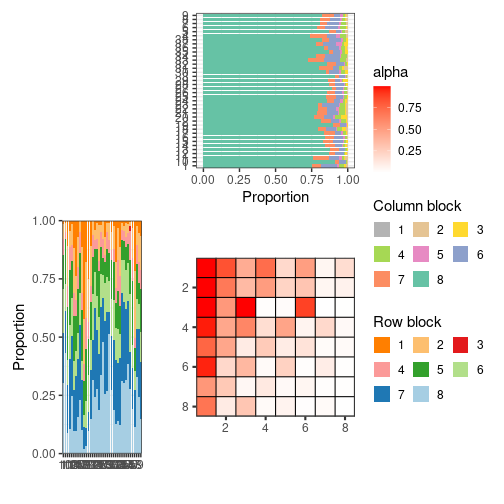
\includegraphics{presentation_dore_files/figure-latex/iid_meso_plot-1.pdf}
\caption{Collection 1 - iid}
\end{figure}

\begin{tabular}{l}
\hline
Networks\\
\hline
arroyo1982\_1+arroyo1982\_2+arroyo3\\
\hline
eberling1999\\
\hline
kato1990\\
\hline
petanidou1991\\
\hline
Junker2013\\
\hline
bartomeus2008\\
\hline
Benadi2013\_1(950m)+Benadi2013\_2(1170m)+Benadi2013\_6(2020m)\\
\hline
Benadi2013\_4(1700m)+Benadi2013\_5(1800m)\\
\hline
Struck1994\\
\hline
Kato2000\\
\hline
Albrecht2010\_49yr+Albrecht2010\_63yr+Albrecht2010\_84yr+Albrecht2010\_109yr+Albrecht2010\_130yr\\
\hline
Baldock2011\_TB+Baldock2011\_JN\\
\hline
Dattilo2016\\
\hline
Devoto2005\_PP+Devoto2005\_AP\\
\hline
Devoto2005\_VT\\
\hline
Devoto2005\_LL+Devoto2005\_CT\\
\hline
Freitas2006\\
\hline
Gibson2006\_TA2\\
\hline
Jedrzejewska2013\_Ochata+Jedrzejewska2013\_Kabaty\\
\hline
MonteroCastano2017\_Albufera+MonteroCastano2017\_Llimpa+MonteroCastano2017\_Tirant\\
\hline
Kehinde2014\_Joostenberg\_Conv+Kehinde2014\_Joostenberg\_Org+Kehinde2014\_Joostenberg\_Nat+Kehinde2014\_Laibach\_Conv+Kehinde2014\_Laibach\_Org+Kehinde2014\_Laibach\_Nat+Kehinde2014\_Spier\_Conv+Kehinde2014\_Spier\_Nat\\
\hline
Pinheiro2008\\
\hline
Watts2016\_Chicon+Watts2016\_Mantanay+Watts2016\_Choquebamba+Watts2016\_Huaran+Watts2016\_Piscacucho+Watts2016\_Poques+Watts2016\_Pumamarca+Watts2016\_Tiaparo+Watts2016\_Yanacocha\\
\hline
Kato1993\\
\hline
KatoMiura1996\\
\hline
Kakutani1990\\
\hline
Inoue1990\\
\hline
Fragoso\_RA2+Fragoso\_RA3+Fragoso\_RD1+Fragoso\_RD3\\
\hline
Souza\_cerrado\\
\hline
Souza\_chaco\\
\hline
Souza\_pantanal\\
\hline
Souza\_vereda\\
\hline
Adedoja2019\\
\hline
Oleques2019\\
\hline
Baldock2019\_Bristol\\
\hline
Baldock2019\_Edinburgh\\
\hline
Baldock2019\_Leeds\\
\hline
Baldock2019\_Reading\\
\hline
\end{tabular}

Pour la collection 2

\begin{figure}
\centering
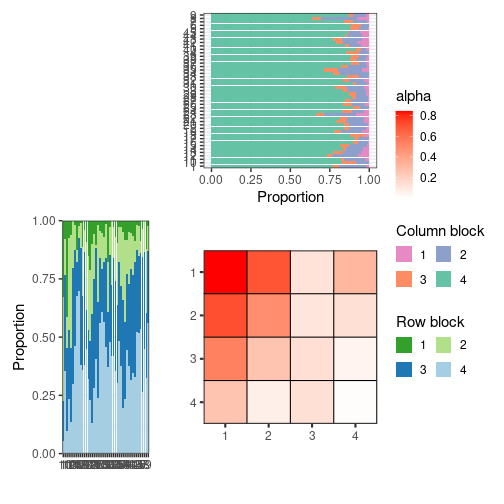
\includegraphics{presentation_dore_files/figure-latex/iid_meso_plot-2.pdf}
\caption{Collection 2 - iid}
\end{figure}

\begin{tabular}{l}
\hline
Networks\\
\hline
dupont2003\\
\hline
herrera1988\\
\hline
inouye1988\\
\hline
medan2002ld\\
\hline
medan2002rb\\
\hline
ramirez1992\\
\hline
ramirez1989\\
\hline
Burkle2013\\
\hline
Olito-Fox2014\\
\hline
Benadi2013\_3(1340m)\\
\hline
Aizen2008\_Challhuaco\_U+Aizen2008\_Challhuaco\_D\\
\hline
Aizen2008\_Cerro Otto\_U+Aizen2008\_Cerro Otto\_D\\
\hline
Aizen2008\_Llao-llao\_U+Aizen2008\_Llao-llao\_D\\
\hline
Chamberlain\_cr1+Chamberlain\_cr2+Chamberlain\_fs1+Chamberlain\_fs2+Chamberlain\_go1+Chamberlain\_go2+Chamberlain\_mm1+Chamberlain\_mm2+Chamberlain\_mz1+Chamberlain\_mz2+Chamberlain\_sm1+Chamberlain\_sm2\\
\hline
Chamberlain\_HLU+Chamberlain\_HLG+Chamberlain\_OKU+Chamberlain\_OKG+Chamberlain\_WLU+Chamberlain\_WLG+Chamberlain\_SOU+Chamberlain\_SOG\\
\hline
Devoto2005\_LQ\\
\hline
Devoto2005\_LT+Devoto2005\_LH\\
\hline
LemusJimenez2003\\
\hline
Lundgren2005\\
\hline
Marrero2013\\
\hline
Trojelsgaard2015\_La Gomera\\
\hline
Trojelsgaard2015\_Gran Canaria\\
\hline
Zackenberg\\
\hline
Yoshihara2008\\
\hline
Fragoso\_RA1+Fragoso\_RD2\\
\hline
PopicThesis\\
\hline
Pornon2017\\
\hline
Orford\_B1+Orford\_B2+Orford\_B3+Orford\_B4+Orford\_B5+Orford\_B10\\
\hline
Orford\_B6+Orford\_B7+Orford\_B8+Orford\_B9\\
\hline
Blumel2016\\
\hline
Kantsa2018\\
\hline
Bennett2018\\
\hline
Adedoja2018b\_baseZone+Adedoja2018b\_MidZone+Adedoja2018b\_HighZone+Adedoja2018b\_PeakZone\\
\hline
CordenizPicanco2018\_NatVeg\\
\hline
CordenizPicanco2018\_ExoFor\\
\hline
Benadi2018\\
\hline
Hackett2019\_NZ\_salt\_marsh+Hackett2019\_NZ\_sand\_dune+Hackett2019\_NZ\_scrub\_coprosma\\
\hline
Jolls2019\\
\hline
Traveset2013\_Fernandina\\
\hline
Traveset2013\_Pinta\\
\hline
Traveset2013\_Santiago\\
\hline
Traveset2013\_SantaCruz\\
\hline
Traveset2013\_SanCristobal\\
\hline
Simanonok2014\\
\hline
Son2019\_a1+Son2019\_a2+Son2019\_a3+Son2019\_a4+Son2019\_a5+Son2019\_a6+Son2019\_a7+Son2019\_a8+Son2019\_F1+Son2019\_F2+Son2019\_F3+Son2019\_F4+Son2019\_F5+Son2019\_F6+Son2019\_F7+Son2019\_F8\\
\hline
\end{tabular}

Pour la collection 3

\begin{figure}
\centering
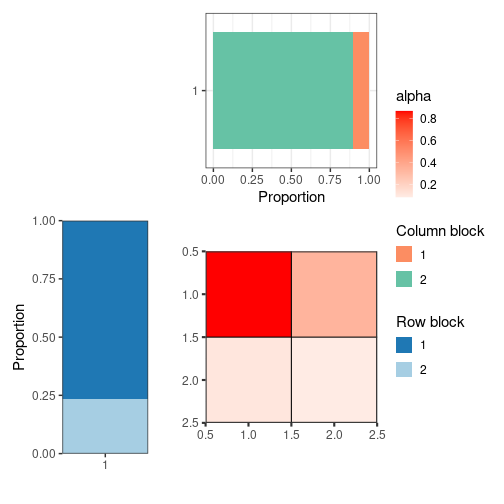
\includegraphics{presentation_dore_files/figure-latex/iid_meso_plot-3.pdf}
\caption{Collection 3 - iid}
\end{figure}

\begin{tabular}{l}
\hline
Networks\\
\hline
small1976\\
\hline
\end{tabular}

Pour la collection 4

\begin{figure}
\centering
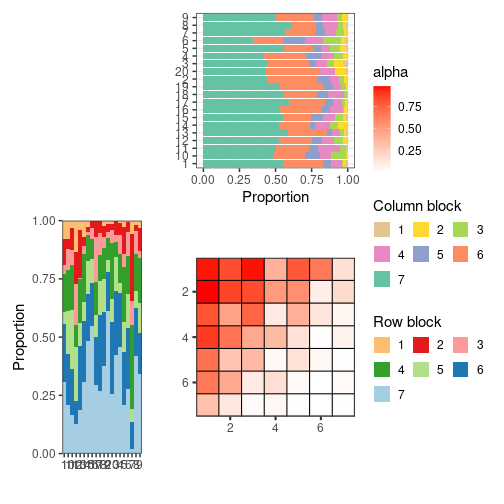
\includegraphics{presentation_dore_files/figure-latex/iid_meso_plot-4.pdf}
\caption{Collection 4 - iid}
\end{figure}

\begin{tabular}{l}
\hline
Networks\\
\hline
smith-ramirez2005\\
\hline
Weiner2011\\
\hline
Kaiser\_control+Kaiser\_restored\\
\hline
Gilarranz2014\_amarante+Gilarranz2014\_barrosa+Gilarranz2014\_cincocerros+Gilarranz2014\_difuntito+Gilarranz2014\_difuntos+Gilarranz2014\_elmorro+Gilarranz2014\_labrava+Gilarranz2014\_lachata+Gilarranz2014\_lapaja+Gilarranz2014\_piedraalta+Gilarranz2014\_vigilancia+Gilarranz2014\_volcan\\
\hline
Kaiser-Bunbury2017\_Bernica+Kaiser-Bunbury2017\_Casse-dent+Kaiser-Bunbury2017\_Copolia+Kaiser-Bunbury2017\_La-Reserve+Kaiser-Bunbury2017\_Rosebelle+Kaiser-Bunbury2017\_Salazie+Kaiser-Bunbury2017\_Tea-Plantation+Kaiser-Bunbury2017\_Trois-Freres\\
\hline
Fang2012\\
\hline
Aizen2008\_Puerto Blest\_U+Aizen2008\_Puerto Blest\_D\\
\hline
Chamberlain\_Site1+Chamberlain\_Site2+Chamberlain\_Site3+Chamberlain\_Site4+Chamberlain\_Site5+Chamberlain\_Site6\\
\hline
Dupont2009\_IsenBjerg+Dupont2009\_Other\\
\hline
Gibson2006\_GA1\\
\hline
Gibson2006\_TA1\\
\hline
LaraRomero2016\_pe?alara\_EP+LaraRomero2016\_pe?alara\_PA+LaraRomero2016\_nevero\_EP+LaraRomero2016\_nevero\_PA\\
\hline
Trojelsgaard2015\_Tenerife Teno Bajo+Trojelsgaard2015\_Tenerife Fasnia\\
\hline
Vanbergen2013\_balfarm+Vanbergen2013\_bridgend+Vanbergen2013\_dalhaikie+Vanbergen2013\_netherton+Vanbergen2013\_backhill+Vanbergen2013\_corntulloch+Vanbergen2013\_allancreich\\
\hline
Pfeiffer\_CNE+Pfeiffer\_CNM+Pfeiffer\_CNT+Pfeiffer\_CPB+Pfeiffer\_CPM+Pfeiffer\_CPR+Pfeiffer\_CPS+Pfeiffer\_M2+Pfeiffer\_RP1+Pfeiffer\_RP2+Pfeiffer\_LM+Pfeiffer\_LO+Pfeiffer\_BD+Pfeiffer\_BH+Pfeiffer\_BS\\
\hline
Carstensen\_Gigante+Carstensen\_Paulino+Carstensen\_Tinkerbell+Carstensen\_Midway+Carstensen\_Cedro+Carstensen\_Elefante+Carstensen\_Soizig\\
\hline
Welti\_ID+Welti\_K1B+Welti\_K4A+Welti\_4B+Welti\_20B+Welti\_20C+Welti\_N1A+Welti\_N1B+Welti\_N4A+Welti\_N4B+Welti\_N20A+Welti\_N20B\\
\hline
Grass2013\_1+Grass2013\_2+Grass2013\_3+Grass2013\_4+Grass2013\_5+Grass2013\_6+Grass2013\_7+Grass2013\_8+Grass2013\_9+Grass2013\_10+Grass2013\_11+Grass2013\_12+Grass2013\_13+Grass2013\_14+Grass2013\_15+Grass2013\_16+Grass2013\_17\\
\hline
Hackett2019\_UK\_sand\_dune+Hackett2019\_UK\_grassland+Hackett2019\_UK\_heathland+Hackett2019\_UK\_woodland+Hackett2019\_UK\_salt\_marsh+Hackett2019\_UK\_scrub\\
\hline
Neli2014\\
\hline
\end{tabular}

Pour la collection 5

\begin{figure}
\centering
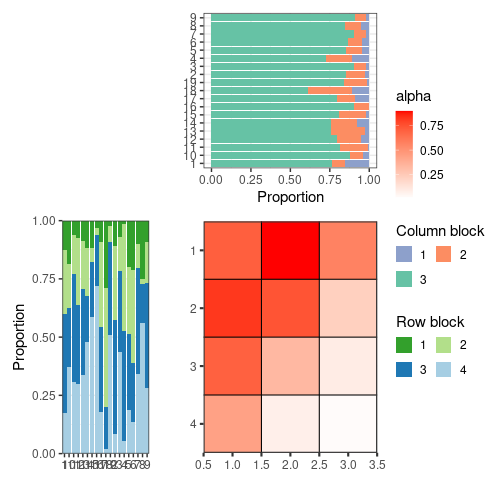
\includegraphics{presentation_dore_files/figure-latex/iid_meso_plot-5.pdf}
\caption{Collection 5 - iid}
\end{figure}

\begin{tabular}{l}
\hline
Networks\\
\hline
olensen2002aig\\
\hline
olensen2002flo\\
\hline
vazquez2002\\
\hline
Shay2016\\
\hline
Gibson2006\_GA2\\
\hline
Gibson2006\_SG\\
\hline
Trojelsgaard2015\_El Hierro\\
\hline
Trojelsgaard2015\_Fuerteventura\\
\hline
Trojelsgaard2015\_Western Sahara\\
\hline
Robinson2018\\
\hline
CordenizPicanco2018\_NatFor\\
\hline
CordenizPicanco2018\_SemiPast\\
\hline
CordenizPicanco2018\_IntPast\\
\hline
Biella2019\\
\hline
Nel2017\\
\hline
Villalobos2019\\
\hline
LaraRomero2019\_blanca+LaraRomero2019\_rajada+LaraRomero2019\_refugio+LaraRomero2019\_torre\\
\hline
Ferrero2013\\
\hline
Sritongchuay2019\_near+Sritongchuay2019\_far\\
\hline
\end{tabular}

Et voici donc les valeurs numériques pour les \(\alpha\) (paramètres de
connectivité).

Pour la collection 1 :
\[\begin{bmatrix} 1 &0.83 &0.43 &0.73 &0.2 &0.5 &0.05 &0.18 \\1 &0.67 &0.36 &0.51 &0.22 &0.3 &0.05 &0.07 \\1 &0.53 &1 &0.01 &0.02 &0.89 &0 &0 \\0.97 &0.45 &0.62 &0.18 &0.47 &0.06 &0.2 &0.03 \\0.76 &0.46 &0.1 &0.27 &0.1 &0.14 &0.02 &0.03 \\0.96 &0.2 &0.37 &0.03 &0.24 &0.01 &0.09 &0.01 \\0.54 &0.28 &0.04 &0.12 &0.03 &0.05 &0.01 &0.01 \\0.69 &0.1 &0.3 &0.02 &0.06 &0.01 &0.03 &0 \\ \end{bmatrix}\]
Pour la collection 2 :
\[\begin{bmatrix} 0.84 &0.69 &0.13 &0.32 \\0.71 &0.49 &0.11 &0.14 \\0.54 &0.26 &0.14 &0.05 \\0.26 &0.07 &0.14 &0.01 \\ \end{bmatrix}\]
Pour la collection 3 :
\[\begin{bmatrix} 0.87 &0.33 \\0.11 &0.09 \\ \end{bmatrix}\] Pour la
collection 4 :
\[\begin{bmatrix} 0.96 &0.83 &0.96 &0.39 &0.8 &0.16 &0.66 \\0.98 &0.86 &0.83 &0.51 &0.56 &0.19 &0.09 \\0.8 &0.46 &0.74 &0.12 &0.4 &0.05 &0.13 \\0.89 &0.69 &0.44 &0.35 &0.15 &0.07 &0.01 \\0.7 &0.29 &0.35 &0.03 &0.15 &0.01 &0.03 \\0.66 &0.43 &0.1 &0.17 &0.03 &0.02 &0 \\0.32 &0.12 &0.02 &0.04 &0 &0 &0 \\ \end{bmatrix}\]
Pour la collection 5 :
\[\begin{bmatrix} 0.71 &0.9 &0.57 &0.83 \\0.74 &0.22 &0.7 &0.33 \\0.09 &0.44 &0.07 &0.02 \\ \end{bmatrix}\]

\hypertarget{ruxe9partition-dans-les-clusters-selon-la-taxonomie}{%
\subsubsection{Répartition dans les clusters selon la
taxonomie}\label{ruxe9partition-dans-les-clusters-selon-la-taxonomie}}

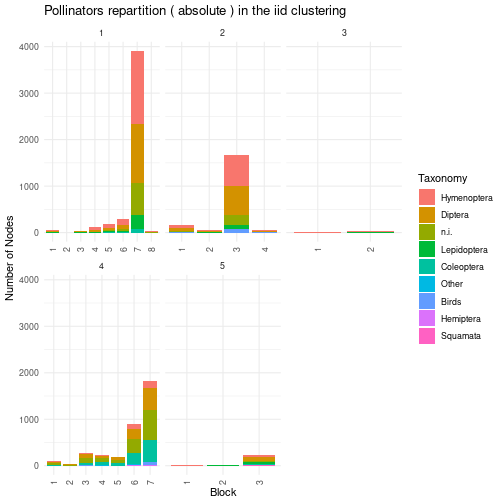
\includegraphics{presentation_dore_files/figure-latex/iid_plot_taxonomy_pollinators-1.pdf}
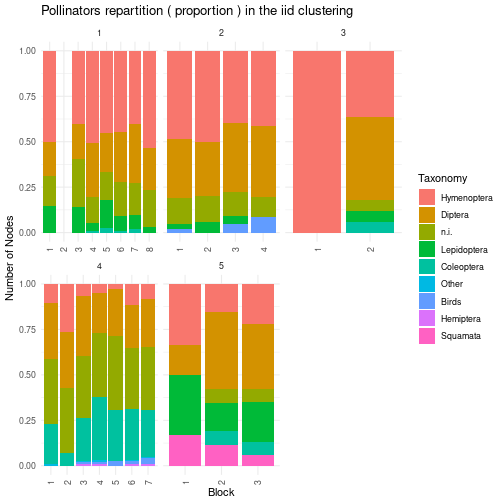
\includegraphics{presentation_dore_files/figure-latex/iid_plot_taxonomy_pollinators-2.pdf}

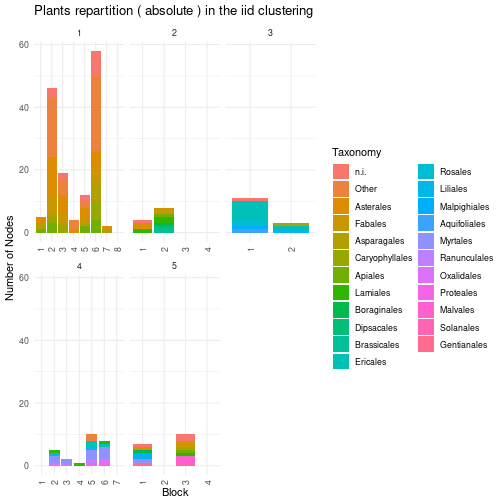
\includegraphics{presentation_dore_files/figure-latex/iid_plot_taxonomy_plants-1.pdf}
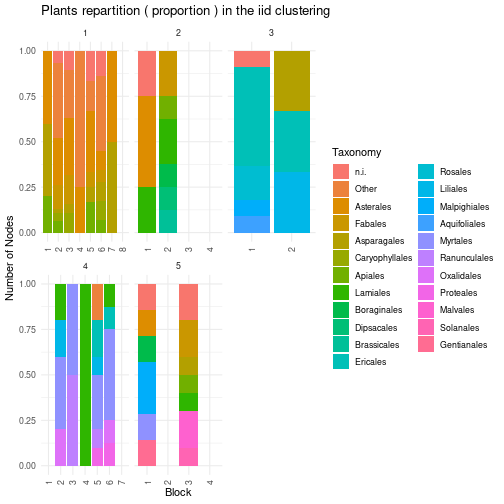
\includegraphics{presentation_dore_files/figure-latex/iid_plot_taxonomy_plants-2.pdf}

\hypertarget{clustering-avec-le-moduxe8le-pi}{%
\subsection{Clustering avec le modèle
pi}\label{clustering-avec-le-moduxe8le-pi}}

Avec le modèle \emph{pi} nous obtenons les 2 collections et les
structures suivantes:

Pour la collection 1

\begin{figure}
\centering
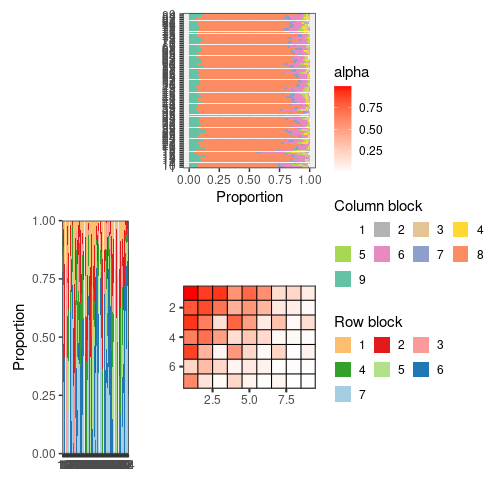
\includegraphics{presentation_dore_files/figure-latex/pi_meso_plot-1.pdf}
\caption{Collection 1 - pi}
\end{figure}

\begin{tabular}{l}
\hline
Networks\\
\hline
arroyo1982\_1+arroyo1982\_2+arroyo3\\
\hline
eberling1999\\
\hline
inouye1988\\
\hline
kato1990\\
\hline
ramirez1992\\
\hline
petanidou1991\\
\hline
ramirez1989\\
\hline
smith-ramirez2005\\
\hline
Junker2013\\
\hline
Kaiser\_control+Kaiser\_restored\\
\hline
bartomeus2008\\
\hline
Olito-Fox2014\\
\hline
Benadi2013\_1(950m)+Benadi2013\_2(1170m)+Benadi2013\_6(2020m)\\
\hline
Benadi2013\_3(1340m)\\
\hline
Benadi2013\_4(1700m)+Benadi2013\_5(1800m)\\
\hline
Kaiser-Bunbury2017\_Bernica+Kaiser-Bunbury2017\_Casse-dent+Kaiser-Bunbury2017\_Copolia+Kaiser-Bunbury2017\_La-Reserve+Kaiser-Bunbury2017\_Rosebelle+Kaiser-Bunbury2017\_Salazie+Kaiser-Bunbury2017\_Tea-Plantation+Kaiser-Bunbury2017\_Trois-Freres\\
\hline
Fang2012\\
\hline
Shay2016\\
\hline
Struck1994\\
\hline
Kato2000\\
\hline
Aizen2008\_Cerro Otto\_U+Aizen2008\_Cerro Otto\_D\\
\hline
Aizen2008\_Llao-llao\_U+Aizen2008\_Llao-llao\_D\\
\hline
Aizen2008\_Puerto Blest\_U+Aizen2008\_Puerto Blest\_D\\
\hline
Albrecht2010\_49yr+Albrecht2010\_63yr+Albrecht2010\_84yr+Albrecht2010\_109yr+Albrecht2010\_130yr\\
\hline
Baldock2011\_TB+Baldock2011\_JN\\
\hline
Chamberlain\_cr1+Chamberlain\_cr2+Chamberlain\_fs1+Chamberlain\_fs2+Chamberlain\_go1+Chamberlain\_go2+Chamberlain\_mm1+Chamberlain\_mm2+Chamberlain\_mz1+Chamberlain\_mz2+Chamberlain\_sm1+Chamberlain\_sm2\\
\hline
Chamberlain\_HLU+Chamberlain\_HLG+Chamberlain\_OKU+Chamberlain\_OKG+Chamberlain\_WLU+Chamberlain\_WLG+Chamberlain\_SOU+Chamberlain\_SOG\\
\hline
Chamberlain\_Site1+Chamberlain\_Site2+Chamberlain\_Site3+Chamberlain\_Site4+Chamberlain\_Site5+Chamberlain\_Site6\\
\hline
Dattilo2016\\
\hline
Devoto2005\_PP+Devoto2005\_AP\\
\hline
Devoto2005\_VT\\
\hline
Devoto2005\_LL+Devoto2005\_CT\\
\hline
Dupont2009\_IsenBjerg+Dupont2009\_Other\\
\hline
Freitas2006\\
\hline
Gibson2006\_TA1\\
\hline
Gibson2006\_TA2\\
\hline
Jedrzejewska2013\_Ochata+Jedrzejewska2013\_Kabaty\\
\hline
LaraRomero2016\_pe?alara\_EP+LaraRomero2016\_pe?alara\_PA+LaraRomero2016\_nevero\_EP+LaraRomero2016\_nevero\_PA\\
\hline
LemusJimenez2003\\
\hline
Marrero2013\\
\hline
MonteroCastano2017\_Albufera+MonteroCastano2017\_Llimpa+MonteroCastano2017\_Tirant\\
\hline
Kehinde2014\_Joostenberg\_Conv+Kehinde2014\_Joostenberg\_Org+Kehinde2014\_Joostenberg\_Nat+Kehinde2014\_Laibach\_Conv+Kehinde2014\_Laibach\_Org+Kehinde2014\_Laibach\_Nat+Kehinde2014\_Spier\_Conv+Kehinde2014\_Spier\_Nat\\
\hline
Pinheiro2008\\
\hline
Trojelsgaard2015\_La Gomera\\
\hline
Trojelsgaard2015\_Tenerife Teno Bajo+Trojelsgaard2015\_Tenerife Fasnia\\
\hline
Vanbergen2013\_balfarm+Vanbergen2013\_bridgend+Vanbergen2013\_dalhaikie+Vanbergen2013\_netherton+Vanbergen2013\_backhill+Vanbergen2013\_corntulloch+Vanbergen2013\_allancreich\\
\hline
Zackenberg\\
\hline
Yoshihara2008\\
\hline
Watts2016\_Chicon+Watts2016\_Mantanay+Watts2016\_Choquebamba+Watts2016\_Huaran+Watts2016\_Piscacucho+Watts2016\_Poques+Watts2016\_Pumamarca+Watts2016\_Tiaparo+Watts2016\_Yanacocha\\
\hline
Kato1993\\
\hline
KatoMiura1996\\
\hline
Kakutani1990\\
\hline
Inoue1990\\
\hline
Fragoso\_RA2+Fragoso\_RA3+Fragoso\_RD1+Fragoso\_RD3\\
\hline
PopicThesis\\
\hline
Pfeiffer\_CNE+Pfeiffer\_CNM+Pfeiffer\_CNT+Pfeiffer\_CPB+Pfeiffer\_CPM+Pfeiffer\_CPR+Pfeiffer\_CPS+Pfeiffer\_M2+Pfeiffer\_RP1+Pfeiffer\_RP2+Pfeiffer\_LM+Pfeiffer\_LO+Pfeiffer\_BD+Pfeiffer\_BH+Pfeiffer\_BS\\
\hline
Carstensen\_Gigante+Carstensen\_Paulino+Carstensen\_Tinkerbell+Carstensen\_Midway+Carstensen\_Cedro+Carstensen\_Elefante+Carstensen\_Soizig\\
\hline
Orford\_B1+Orford\_B2+Orford\_B3+Orford\_B4+Orford\_B5+Orford\_B10\\
\hline
Orford\_B6+Orford\_B7+Orford\_B8+Orford\_B9\\
\hline
Blumel2016\\
\hline
Welti\_ID+Welti\_K1B+Welti\_K4A+Welti\_4B+Welti\_20B+Welti\_20C+Welti\_N1A+Welti\_N1B+Welti\_N4A+Welti\_N4B+Welti\_N20A+Welti\_N20B\\
\hline
Souza\_cerrado\\
\hline
Souza\_chaco\\
\hline
Souza\_pantanal\\
\hline
Souza\_vereda\\
\hline
Grass2013\_1+Grass2013\_2+Grass2013\_3+Grass2013\_4+Grass2013\_5+Grass2013\_6+Grass2013\_7+Grass2013\_8+Grass2013\_9+Grass2013\_10+Grass2013\_11+Grass2013\_12+Grass2013\_13+Grass2013\_14+Grass2013\_15+Grass2013\_16+Grass2013\_17\\
\hline
Bennett2018\\
\hline
Adedoja2018b\_baseZone+Adedoja2018b\_MidZone+Adedoja2018b\_HighZone+Adedoja2018b\_PeakZone\\
\hline
Adedoja2019\\
\hline
CordenizPicanco2018\_NatVeg\\
\hline
Benadi2018\\
\hline
Hackett2019\_NZ\_salt\_marsh+Hackett2019\_NZ\_sand\_dune+Hackett2019\_NZ\_scrub\_coprosma\\
\hline
Oleques2019\\
\hline
Jolls2019\\
\hline
Traveset2013\_Fernandina\\
\hline
Traveset2013\_Santiago\\
\hline
Traveset2013\_SantaCruz\\
\hline
Traveset2013\_SanCristobal\\
\hline
Simanonok2014\\
\hline
Son2019\_a1+Son2019\_a2+Son2019\_a3+Son2019\_a4+Son2019\_a5+Son2019\_a6+Son2019\_a7+Son2019\_a8+Son2019\_F1+Son2019\_F2+Son2019\_F3+Son2019\_F4+Son2019\_F5+Son2019\_F6+Son2019\_F7+Son2019\_F8\\
\hline
Baldock2019\_Bristol\\
\hline
Baldock2019\_Edinburgh\\
\hline
Baldock2019\_Leeds\\
\hline
Baldock2019\_Reading\\
\hline
\end{tabular}

Pour la collection 2

\begin{figure}
\centering
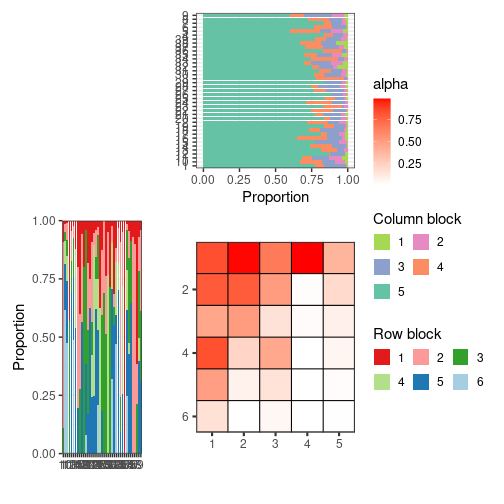
\includegraphics{presentation_dore_files/figure-latex/pi_meso_plot-2.pdf}
\caption{Collection 2 - pi}
\end{figure}

\begin{tabular}{l}
\hline
Networks\\
\hline
dupont2003\\
\hline
herrera1988\\
\hline
medan2002ld\\
\hline
medan2002rb\\
\hline
olensen2002aig\\
\hline
olensen2002flo\\
\hline
small1976\\
\hline
vazquez2002\\
\hline
Burkle2013\\
\hline
Weiner2011\\
\hline
Gilarranz2014\_amarante+Gilarranz2014\_barrosa+Gilarranz2014\_cincocerros+Gilarranz2014\_difuntito+Gilarranz2014\_difuntos+Gilarranz2014\_elmorro+Gilarranz2014\_labrava+Gilarranz2014\_lachata+Gilarranz2014\_lapaja+Gilarranz2014\_piedraalta+Gilarranz2014\_vigilancia+Gilarranz2014\_volcan\\
\hline
Aizen2008\_Challhuaco\_U+Aizen2008\_Challhuaco\_D\\
\hline
Devoto2005\_LQ\\
\hline
Devoto2005\_LT+Devoto2005\_LH\\
\hline
Gibson2006\_GA1\\
\hline
Gibson2006\_GA2\\
\hline
Gibson2006\_SG\\
\hline
Lundgren2005\\
\hline
Trojelsgaard2015\_El Hierro\\
\hline
Trojelsgaard2015\_Gran Canaria\\
\hline
Trojelsgaard2015\_Fuerteventura\\
\hline
Trojelsgaard2015\_Western Sahara\\
\hline
Fragoso\_RA1+Fragoso\_RD2\\
\hline
Pornon2017\\
\hline
Kantsa2018\\
\hline
Robinson2018\\
\hline
CordenizPicanco2018\_NatFor\\
\hline
CordenizPicanco2018\_ExoFor\\
\hline
CordenizPicanco2018\_SemiPast\\
\hline
CordenizPicanco2018\_IntPast\\
\hline
Hackett2019\_UK\_sand\_dune+Hackett2019\_UK\_grassland+Hackett2019\_UK\_heathland+Hackett2019\_UK\_woodland+Hackett2019\_UK\_salt\_marsh+Hackett2019\_UK\_scrub\\
\hline
Biella2019\\
\hline
Nel2017\\
\hline
Villalobos2019\\
\hline
LaraRomero2019\_blanca+LaraRomero2019\_rajada+LaraRomero2019\_refugio+LaraRomero2019\_torre\\
\hline
Traveset2013\_Pinta\\
\hline
Ferrero2013\\
\hline
Neli2014\\
\hline
Sritongchuay2019\_near+Sritongchuay2019\_far\\
\hline
\end{tabular}

Et voici donc les valeurs numériques pour les \(\alpha\) (paramètres de
connectivité).

Pour la collection 1 :
\[\begin{bmatrix} 1 &0.9 &0.92 &0.55 &0.75 &0.57 &0.17 \\0.1 &0.21 &0.81 &0.86 &0.7 &0.4 &0.54 \\0.38 &0.12 &0.03 &0.09 &0.92 &0.65 &0.17 \\0.76 &0.5 &0.1 &0.33 &0.17 &0.04 &0.65 \\0.71 &0.5 &0.18 &0.28 &0.19 &0.04 &0.01 \\0.03 &0.89 &0.4 &0.05 &0.53 &0.2 &0.03 \\0.22 &0.07 &0.01 &0.22 &0.35 &0.21 &0.06 \\0.11 &0.07 &0.01 &0.01 &0.01 &0.6 &0.15 \\0.02 &0.21 &0.06 &0.01 &0.06 &0.01 &0 \\ \end{bmatrix}\]
Pour la collection 2 :
\[\begin{bmatrix} 0.84 &0.99 &0.66 &0.99 &0.38 &0.79 \\0.79 &0.5 &0.01 &0.19 &0.46 &0.51 \\0.15 &0.02 &0.08 &0.83 &0.22 &0.44 \\0 &0.05 &0.49 &0.07 &0.15 &0 \\0.01 &0.16 &0 &0.04 &0 &0 \\ \end{bmatrix}\]

\hypertarget{ruxe9partition-dans-les-clusters-selon-la-taxonomie-1}{%
\subsubsection{Répartition dans les clusters selon la
taxonomie}\label{ruxe9partition-dans-les-clusters-selon-la-taxonomie-1}}

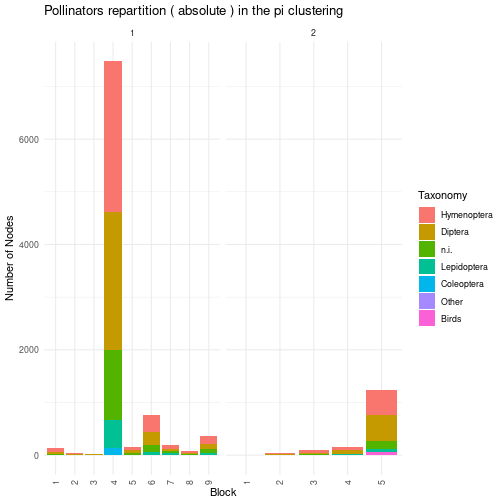
\includegraphics{presentation_dore_files/figure-latex/pi_plot_taxonomy_pollinators-1.pdf}
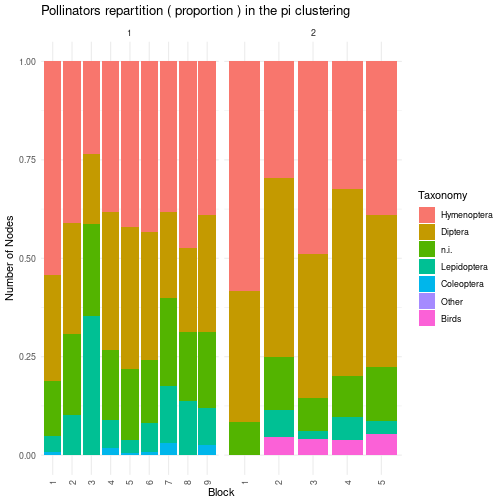
\includegraphics{presentation_dore_files/figure-latex/pi_plot_taxonomy_pollinators-2.pdf}

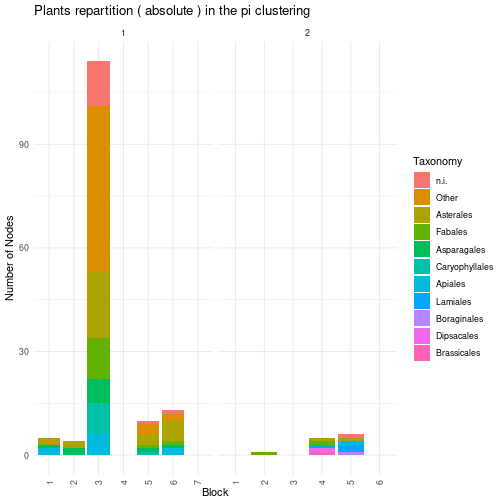
\includegraphics{presentation_dore_files/figure-latex/pi_plot_taxonomy_plants-1.pdf}
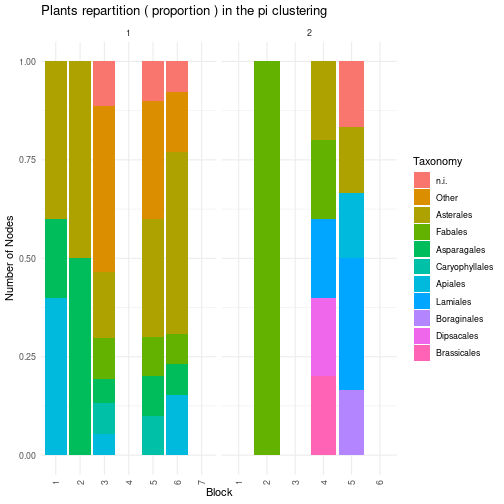
\includegraphics{presentation_dore_files/figure-latex/pi_plot_taxonomy_plants-2.pdf}

\hypertarget{clustering-avec-le-moduxe8le-rho}{%
\subsection{Clustering avec le modèle
rho}\label{clustering-avec-le-moduxe8le-rho}}

Avec le modèle \emph{rho} nous obtenons les 1 collections et les
structures suivantes:

Pour la collection 1

\begin{figure}
\centering
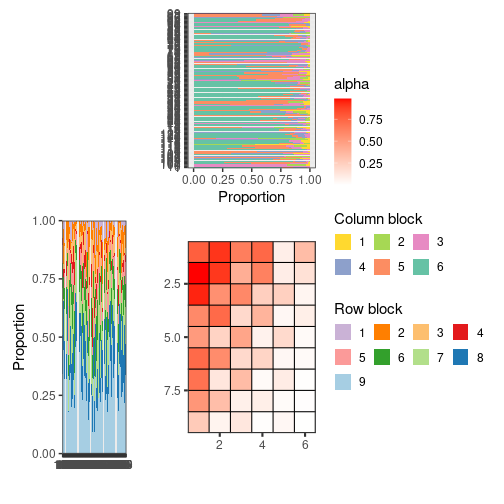
\includegraphics{presentation_dore_files/figure-latex/rho_meso_plot-1.pdf}
\caption{Collection 1 - rho}
\end{figure}

\begin{tabular}{l}
\hline
Networks\\
\hline
arroyo1982\_1+arroyo1982\_2+arroyo3\\
\hline
dupont2003\\
\hline
eberling1999\\
\hline
herrera1988\\
\hline
inouye1988\\
\hline
kato1990\\
\hline
medan2002ld\\
\hline
medan2002rb\\
\hline
olensen2002aig\\
\hline
olensen2002flo\\
\hline
ramirez1992\\
\hline
small1976\\
\hline
vazquez2002\\
\hline
petanidou1991\\
\hline
ramirez1989\\
\hline
smith-ramirez2005\\
\hline
Burkle2013\\
\hline
Junker2013\\
\hline
Weiner2011\\
\hline
Kaiser\_control+Kaiser\_restored\\
\hline
bartomeus2008\\
\hline
Olito-Fox2014\\
\hline
Gilarranz2014\_amarante+Gilarranz2014\_barrosa+Gilarranz2014\_cincocerros+Gilarranz2014\_difuntito+Gilarranz2014\_difuntos+Gilarranz2014\_elmorro+Gilarranz2014\_labrava+Gilarranz2014\_lachata+Gilarranz2014\_lapaja+Gilarranz2014\_piedraalta+Gilarranz2014\_vigilancia+Gilarranz2014\_volcan\\
\hline
Benadi2013\_1(950m)+Benadi2013\_2(1170m)+Benadi2013\_6(2020m)\\
\hline
Benadi2013\_3(1340m)\\
\hline
Benadi2013\_4(1700m)+Benadi2013\_5(1800m)\\
\hline
Kaiser-Bunbury2017\_Bernica+Kaiser-Bunbury2017\_Casse-dent+Kaiser-Bunbury2017\_Copolia+Kaiser-Bunbury2017\_La-Reserve+Kaiser-Bunbury2017\_Rosebelle+Kaiser-Bunbury2017\_Salazie+Kaiser-Bunbury2017\_Tea-Plantation+Kaiser-Bunbury2017\_Trois-Freres\\
\hline
Fang2012\\
\hline
Shay2016\\
\hline
Struck1994\\
\hline
Kato2000\\
\hline
Aizen2008\_Challhuaco\_U+Aizen2008\_Challhuaco\_D\\
\hline
Aizen2008\_Cerro Otto\_U+Aizen2008\_Cerro Otto\_D\\
\hline
Aizen2008\_Llao-llao\_U+Aizen2008\_Llao-llao\_D\\
\hline
Aizen2008\_Puerto Blest\_U+Aizen2008\_Puerto Blest\_D\\
\hline
Albrecht2010\_49yr+Albrecht2010\_63yr+Albrecht2010\_84yr+Albrecht2010\_109yr+Albrecht2010\_130yr\\
\hline
Baldock2011\_TB+Baldock2011\_JN\\
\hline
Chamberlain\_cr1+Chamberlain\_cr2+Chamberlain\_fs1+Chamberlain\_fs2+Chamberlain\_go1+Chamberlain\_go2+Chamberlain\_mm1+Chamberlain\_mm2+Chamberlain\_mz1+Chamberlain\_mz2+Chamberlain\_sm1+Chamberlain\_sm2\\
\hline
Chamberlain\_HLU+Chamberlain\_HLG+Chamberlain\_OKU+Chamberlain\_OKG+Chamberlain\_WLU+Chamberlain\_WLG+Chamberlain\_SOU+Chamberlain\_SOG\\
\hline
Chamberlain\_Site1+Chamberlain\_Site2+Chamberlain\_Site3+Chamberlain\_Site4+Chamberlain\_Site5+Chamberlain\_Site6\\
\hline
Dattilo2016\\
\hline
Devoto2005\_LQ\\
\hline
Devoto2005\_PP+Devoto2005\_AP\\
\hline
Devoto2005\_LT+Devoto2005\_LH\\
\hline
Devoto2005\_VT\\
\hline
Devoto2005\_LL+Devoto2005\_CT\\
\hline
Dupont2009\_IsenBjerg+Dupont2009\_Other\\
\hline
Freitas2006\\
\hline
Gibson2006\_GA1\\
\hline
Gibson2006\_GA2\\
\hline
Gibson2006\_SG\\
\hline
Gibson2006\_TA1\\
\hline
Gibson2006\_TA2\\
\hline
Jedrzejewska2013\_Ochata+Jedrzejewska2013\_Kabaty\\
\hline
LaraRomero2016\_pe?alara\_EP+LaraRomero2016\_pe?alara\_PA+LaraRomero2016\_nevero\_EP+LaraRomero2016\_nevero\_PA\\
\hline
LemusJimenez2003\\
\hline
Lundgren2005\\
\hline
Marrero2013\\
\hline
MonteroCastano2017\_Albufera+MonteroCastano2017\_Llimpa+MonteroCastano2017\_Tirant\\
\hline
Kehinde2014\_Joostenberg\_Conv+Kehinde2014\_Joostenberg\_Org+Kehinde2014\_Joostenberg\_Nat+Kehinde2014\_Laibach\_Conv+Kehinde2014\_Laibach\_Org+Kehinde2014\_Laibach\_Nat+Kehinde2014\_Spier\_Conv+Kehinde2014\_Spier\_Nat\\
\hline
Pinheiro2008\\
\hline
Trojelsgaard2015\_El Hierro\\
\hline
Trojelsgaard2015\_La Gomera\\
\hline
Trojelsgaard2015\_Gran Canaria\\
\hline
Trojelsgaard2015\_Fuerteventura\\
\hline
Trojelsgaard2015\_Tenerife Teno Bajo+Trojelsgaard2015\_Tenerife Fasnia\\
\hline
Trojelsgaard2015\_Western Sahara\\
\hline
Vanbergen2013\_balfarm+Vanbergen2013\_bridgend+Vanbergen2013\_dalhaikie+Vanbergen2013\_netherton+Vanbergen2013\_backhill+Vanbergen2013\_corntulloch+Vanbergen2013\_allancreich\\
\hline
Zackenberg\\
\hline
Yoshihara2008\\
\hline
Watts2016\_Chicon+Watts2016\_Mantanay+Watts2016\_Choquebamba+Watts2016\_Huaran+Watts2016\_Piscacucho+Watts2016\_Poques+Watts2016\_Pumamarca+Watts2016\_Tiaparo+Watts2016\_Yanacocha\\
\hline
Kato1993\\
\hline
KatoMiura1996\\
\hline
Kakutani1990\\
\hline
Inoue1990\\
\hline
Fragoso\_RA1+Fragoso\_RD2\\
\hline
Fragoso\_RA2+Fragoso\_RA3+Fragoso\_RD1+Fragoso\_RD3\\
\hline
PopicThesis\\
\hline
Pfeiffer\_CNE+Pfeiffer\_CNM+Pfeiffer\_CNT+Pfeiffer\_CPB+Pfeiffer\_CPM+Pfeiffer\_CPR+Pfeiffer\_CPS+Pfeiffer\_M2+Pfeiffer\_RP1+Pfeiffer\_RP2+Pfeiffer\_LM+Pfeiffer\_LO+Pfeiffer\_BD+Pfeiffer\_BH+Pfeiffer\_BS\\
\hline
Carstensen\_Gigante+Carstensen\_Paulino+Carstensen\_Tinkerbell+Carstensen\_Midway+Carstensen\_Cedro+Carstensen\_Elefante+Carstensen\_Soizig\\
\hline
Pornon2017\\
\hline
Orford\_B1+Orford\_B2+Orford\_B3+Orford\_B4+Orford\_B5+Orford\_B10\\
\hline
Orford\_B6+Orford\_B7+Orford\_B8+Orford\_B9\\
\hline
Blumel2016\\
\hline
Welti\_ID+Welti\_K1B+Welti\_K4A+Welti\_4B+Welti\_20B+Welti\_20C+Welti\_N1A+Welti\_N1B+Welti\_N4A+Welti\_N4B+Welti\_N20A+Welti\_N20B\\
\hline
Kantsa2018\\
\hline
Souza\_cerrado\\
\hline
Souza\_chaco\\
\hline
Souza\_pantanal\\
\hline
Souza\_vereda\\
\hline
Grass2013\_1+Grass2013\_2+Grass2013\_3+Grass2013\_4+Grass2013\_5+Grass2013\_6+Grass2013\_7+Grass2013\_8+Grass2013\_9+Grass2013\_10+Grass2013\_11+Grass2013\_12+Grass2013\_13+Grass2013\_14+Grass2013\_15+Grass2013\_16+Grass2013\_17\\
\hline
Robinson2018\\
\hline
Bennett2018\\
\hline
Adedoja2018b\_baseZone+Adedoja2018b\_MidZone+Adedoja2018b\_HighZone+Adedoja2018b\_PeakZone\\
\hline
Adedoja2019\\
\hline
CordenizPicanco2018\_NatFor\\
\hline
CordenizPicanco2018\_NatVeg\\
\hline
CordenizPicanco2018\_ExoFor\\
\hline
CordenizPicanco2018\_SemiPast\\
\hline
CordenizPicanco2018\_IntPast\\
\hline
Benadi2018\\
\hline
Hackett2019\_NZ\_salt\_marsh+Hackett2019\_NZ\_sand\_dune+Hackett2019\_NZ\_scrub\_coprosma\\
\hline
Hackett2019\_UK\_sand\_dune+Hackett2019\_UK\_grassland+Hackett2019\_UK\_heathland+Hackett2019\_UK\_woodland+Hackett2019\_UK\_salt\_marsh+Hackett2019\_UK\_scrub\\
\hline
Oleques2019\\
\hline
Biella2019\\
\hline
Jolls2019\\
\hline
Nel2017\\
\hline
Villalobos2019\\
\hline
LaraRomero2019\_blanca+LaraRomero2019\_rajada+LaraRomero2019\_refugio+LaraRomero2019\_torre\\
\hline
Traveset2013\_Fernandina\\
\hline
Traveset2013\_Pinta\\
\hline
Traveset2013\_Santiago\\
\hline
Traveset2013\_SantaCruz\\
\hline
Traveset2013\_SanCristobal\\
\hline
Ferrero2013\\
\hline
Simanonok2014\\
\hline
Son2019\_a1+Son2019\_a2+Son2019\_a3+Son2019\_a4+Son2019\_a5+Son2019\_a6+Son2019\_a7+Son2019\_a8+Son2019\_F1+Son2019\_F2+Son2019\_F3+Son2019\_F4+Son2019\_F5+Son2019\_F6+Son2019\_F7+Son2019\_F8\\
\hline
Neli2014\\
\hline
Sritongchuay2019\_near+Sritongchuay2019\_far\\
\hline
Baldock2019\_Bristol\\
\hline
Baldock2019\_Edinburgh\\
\hline
Baldock2019\_Leeds\\
\hline
Baldock2019\_Reading\\
\hline
\end{tabular}

Et voici donc les valeurs numériques pour les \(\alpha\) (paramètres de
connectivité).

Pour la collection 1 :
\[\begin{bmatrix} 0.77 &0.91 &0.64 &0.73 &0.09 &0.34 &0.98 &0.9 &0.41 \\0.63 &0.09 &0.15 &0.94 &0.56 &0.6 &0.25 &0.24 &0.05 \\0.59 &0.73 &0.19 &0.38 &0.04 &0.09 &0.51 &0.22 &0.46 \\0.07 &0.19 &0.02 &0.73 &0.58 &0.2 &0.22 &0.04 &0.03 \\0.69 &0.13 &0.34 &0.03 &0.1 &0.01 &0.53 &0.33 &0.08 \\0.09 &0.02 &0.01 &0.27 &0.06 &0.12 &0.01 &0.04 &0 \\ \end{bmatrix}\]

\hypertarget{ruxe9partition-dans-les-clusters-selon-la-taxonomie-2}{%
\subsubsection{Répartition dans les clusters selon la
taxonomie}\label{ruxe9partition-dans-les-clusters-selon-la-taxonomie-2}}

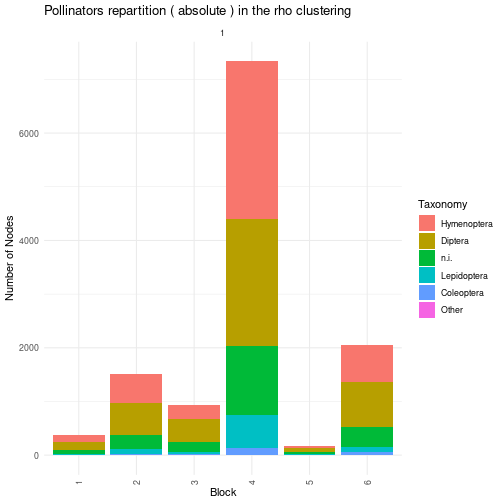
\includegraphics{presentation_dore_files/figure-latex/rho_plot_taxonomy_pollinators-1.pdf}
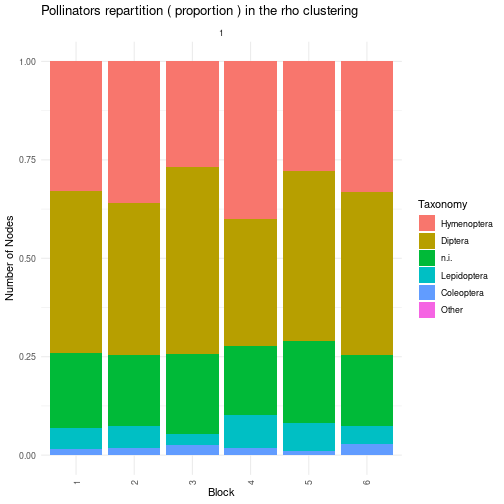
\includegraphics{presentation_dore_files/figure-latex/rho_plot_taxonomy_pollinators-2.pdf}

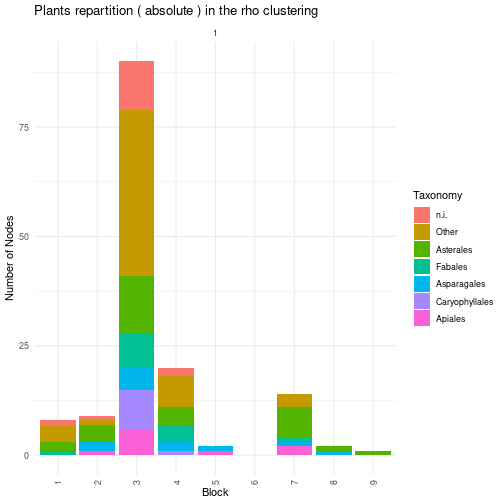
\includegraphics{presentation_dore_files/figure-latex/rho_plot_taxonomy_plants-1.pdf}
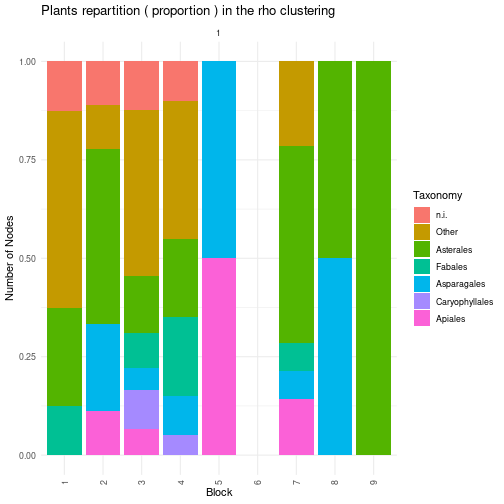
\includegraphics{presentation_dore_files/figure-latex/rho_plot_taxonomy_plants-2.pdf}

\hypertarget{clustering-avec-le-moduxe8le-pirho}{%
\subsection{Clustering avec le modèle
pirho}\label{clustering-avec-le-moduxe8le-pirho}}

Avec le modèle \emph{pirho} nous obtenons les 15 collections et les
structures suivantes:

Pour la collection 1

\begin{figure}
\centering
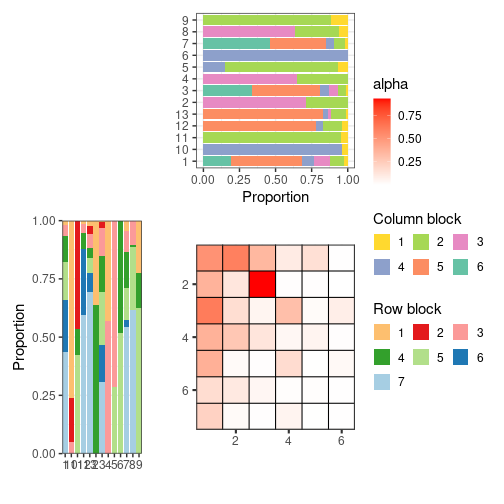
\includegraphics{presentation_dore_files/figure-latex/pirho_meso_plot-1.pdf}
\caption{Collection 1 - pirho}
\end{figure}

\begin{tabular}{l}
\hline
Networks\\
\hline
arroyo1982\_1+arroyo1982\_2+arroyo3\\
\hline
dupont2003\\
\hline
petanidou1991\\
\hline
Aizen2008\_Challhuaco\_U+Aizen2008\_Challhuaco\_D\\
\hline
Aizen2008\_Llao-llao\_U+Aizen2008\_Llao-llao\_D\\
\hline
Jedrzejewska2013\_Ochata+Jedrzejewska2013\_Kabaty\\
\hline
Pinheiro2008\\
\hline
Souza\_pantanal\\
\hline
Robinson2018\\
\hline
Jolls2019\\
\hline
Traveset2013\_Fernandina\\
\hline
Baldock2019\_Leeds\\
\hline
Baldock2019\_Reading\\
\hline
\end{tabular}

Pour la collection 2

\begin{figure}
\centering
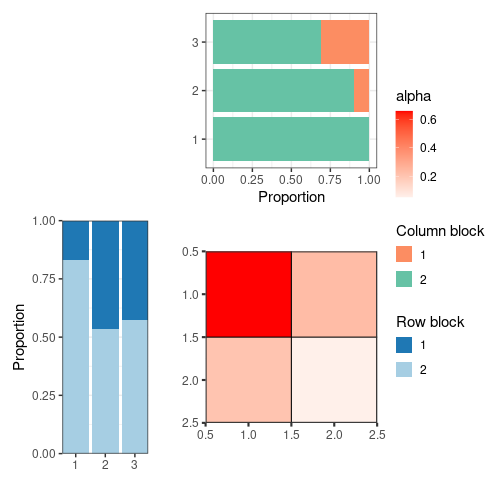
\includegraphics{presentation_dore_files/figure-latex/pirho_meso_plot-2.pdf}
\caption{Collection 2 - pirho}
\end{figure}

\begin{tabular}{l}
\hline
Networks\\
\hline
Benadi2013\_3(1340m)\\
\hline
Trojelsgaard2015\_La Gomera\\
\hline
CordenizPicanco2018\_SemiPast\\
\hline
\end{tabular}

Pour la collection 3

\begin{figure}
\centering
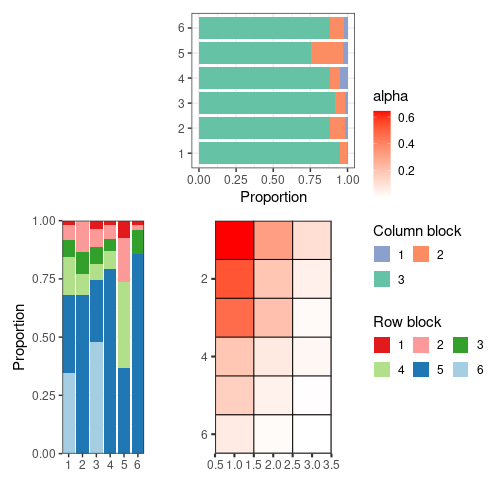
\includegraphics{presentation_dore_files/figure-latex/pirho_meso_plot-3.pdf}
\caption{Collection 3 - pirho}
\end{figure}

\begin{tabular}{l}
\hline
Networks\\
\hline
Kato2000\\
\hline
Freitas2006\\
\hline
Inoue1990\\
\hline
Souza\_cerrado\\
\hline
Adedoja2019\\
\hline
Baldock2019\_Bristol\\
\hline
\end{tabular}

Pour la collection 4

\begin{figure}
\centering
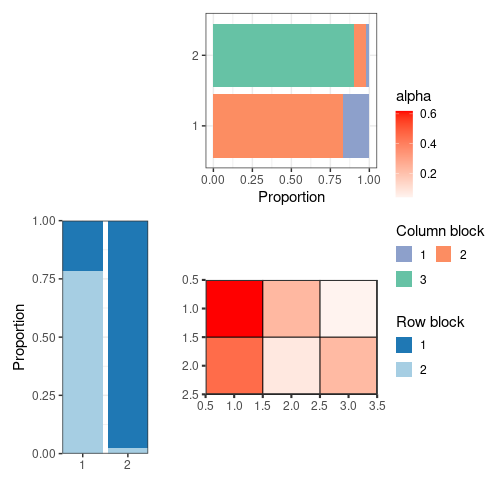
\includegraphics{presentation_dore_files/figure-latex/pirho_meso_plot-4.pdf}
\caption{Collection 4 - pirho}
\end{figure}

\begin{tabular}{l}
\hline
Networks\\
\hline
Aizen2008\_Puerto Blest\_U+Aizen2008\_Puerto Blest\_D\\
\hline
LemusJimenez2003\\
\hline
\end{tabular}

Pour la collection 5

\begin{figure}
\centering
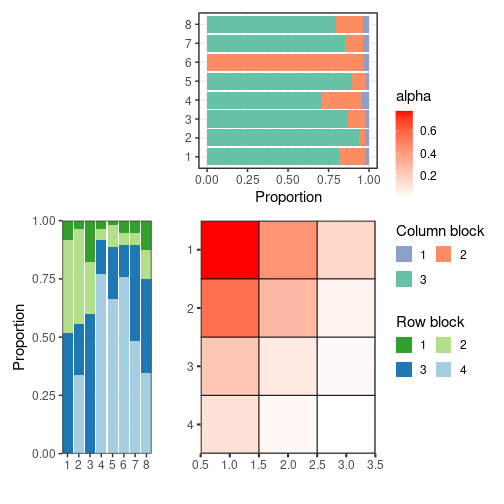
\includegraphics{presentation_dore_files/figure-latex/pirho_meso_plot-5.pdf}
\caption{Collection 5 - pirho}
\end{figure}

\begin{tabular}{l}
\hline
Networks\\
\hline
inouye1988\\
\hline
Junker2013\\
\hline
Kehinde2014\_Joostenberg\_Conv+Kehinde2014\_Joostenberg\_Org+Kehinde2014\_Joostenberg\_Nat+Kehinde2014\_Laibach\_Conv+Kehinde2014\_Laibach\_Org+Kehinde2014\_Laibach\_Nat+Kehinde2014\_Spier\_Conv+Kehinde2014\_Spier\_Nat\\
\hline
Watts2016\_Chicon+Watts2016\_Mantanay+Watts2016\_Choquebamba+Watts2016\_Huaran+Watts2016\_Piscacucho+Watts2016\_Poques+Watts2016\_Pumamarca+Watts2016\_Tiaparo+Watts2016\_Yanacocha\\
\hline
Kakutani1990\\
\hline
Fragoso\_RA1+Fragoso\_RD2\\
\hline
Souza\_chaco\\
\hline
Oleques2019\\
\hline
\end{tabular}

Pour la collection 6

\begin{figure}
\centering
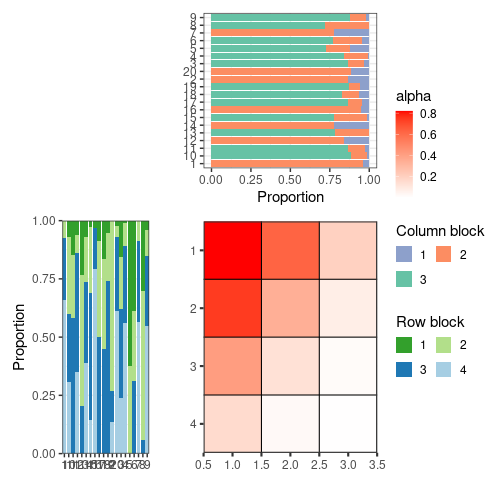
\includegraphics{presentation_dore_files/figure-latex/pirho_meso_plot-6.pdf}
\caption{Collection 6 - pirho}
\end{figure}

\begin{tabular}{l}
\hline
Networks\\
\hline
medan2002ld\\
\hline
small1976\\
\hline
smith-ramirez2005\\
\hline
Benadi2013\_1(950m)+Benadi2013\_2(1170m)+Benadi2013\_6(2020m)\\
\hline
Shay2016\\
\hline
Aizen2008\_Cerro Otto\_U+Aizen2008\_Cerro Otto\_D\\
\hline
Lundgren2005\\
\hline
Zackenberg\\
\hline
Carstensen\_Gigante+Carstensen\_Paulino+Carstensen\_Tinkerbell+Carstensen\_Midway+Carstensen\_Cedro+Carstensen\_Elefante+Carstensen\_Soizig\\
\hline
Welti\_ID+Welti\_K1B+Welti\_K4A+Welti\_4B+Welti\_20B+Welti\_20C+Welti\_N1A+Welti\_N1B+Welti\_N4A+Welti\_N4B+Welti\_N20A+Welti\_N20B\\
\hline
Bennett2018\\
\hline
CordenizPicanco2018\_NatFor\\
\hline
CordenizPicanco2018\_ExoFor\\
\hline
CordenizPicanco2018\_IntPast\\
\hline
Benadi2018\\
\hline
Villalobos2019\\
\hline
Traveset2013\_Santiago\\
\hline
Traveset2013\_SantaCruz\\
\hline
Son2019\_a1+Son2019\_a2+Son2019\_a3+Son2019\_a4+Son2019\_a5+Son2019\_a6+Son2019\_a7+Son2019\_a8+Son2019\_F1+Son2019\_F2+Son2019\_F3+Son2019\_F4+Son2019\_F5+Son2019\_F6+Son2019\_F7+Son2019\_F8\\
\hline
Sritongchuay2019\_near+Sritongchuay2019\_far\\
\hline
\end{tabular}

Pour la collection 7

\begin{figure}
\centering
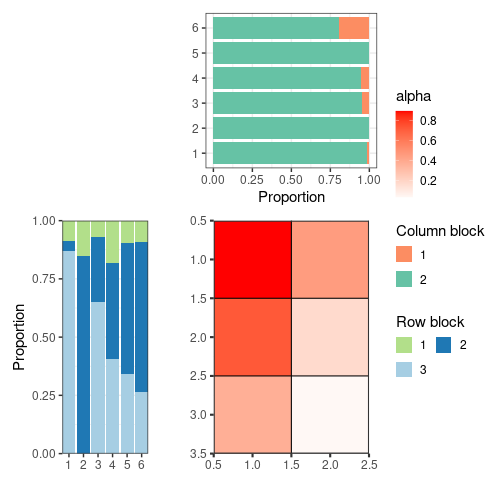
\includegraphics{presentation_dore_files/figure-latex/pirho_meso_plot-7.pdf}
\caption{Collection 7 - pirho}
\end{figure}

\begin{tabular}{l}
\hline
Networks\\
\hline
medan2002rb\\
\hline
olensen2002flo\\
\hline
vazquez2002\\
\hline
Trojelsgaard2015\_Gran Canaria\\
\hline
Trojelsgaard2015\_Western Sahara\\
\hline
LaraRomero2019\_blanca+LaraRomero2019\_rajada+LaraRomero2019\_refugio+LaraRomero2019\_torre\\
\hline
\end{tabular}

Pour la collection 8

\begin{figure}
\centering
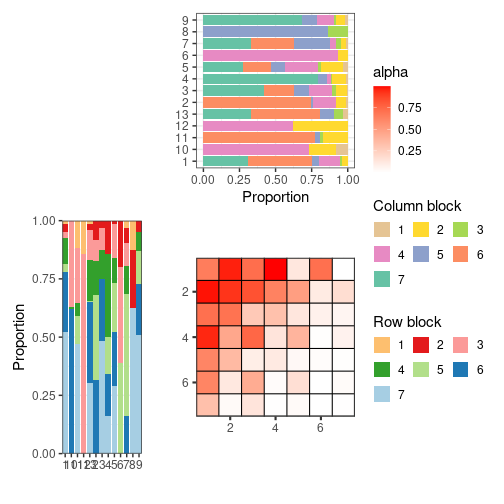
\includegraphics{presentation_dore_files/figure-latex/pirho_meso_plot-8.pdf}
\caption{Collection 8 - pirho}
\end{figure}

\begin{tabular}{l}
\hline
Networks\\
\hline
Weiner2011\\
\hline
Kaiser\_control+Kaiser\_restored\\
\hline
Gilarranz2014\_amarante+Gilarranz2014\_barrosa+Gilarranz2014\_cincocerros+Gilarranz2014\_difuntito+Gilarranz2014\_difuntos+Gilarranz2014\_elmorro+Gilarranz2014\_labrava+Gilarranz2014\_lachata+Gilarranz2014\_lapaja+Gilarranz2014\_piedraalta+Gilarranz2014\_vigilancia+Gilarranz2014\_volcan\\
\hline
Kaiser-Bunbury2017\_Bernica+Kaiser-Bunbury2017\_Casse-dent+Kaiser-Bunbury2017\_Copolia+Kaiser-Bunbury2017\_La-Reserve+Kaiser-Bunbury2017\_Rosebelle+Kaiser-Bunbury2017\_Salazie+Kaiser-Bunbury2017\_Tea-Plantation+Kaiser-Bunbury2017\_Trois-Freres\\
\hline
Fang2012\\
\hline
Gibson2006\_SG\\
\hline
Gibson2006\_TA1\\
\hline
Trojelsgaard2015\_Fuerteventura\\
\hline
Pfeiffer\_CNE+Pfeiffer\_CNM+Pfeiffer\_CNT+Pfeiffer\_CPB+Pfeiffer\_CPM+Pfeiffer\_CPR+Pfeiffer\_CPS+Pfeiffer\_M2+Pfeiffer\_RP1+Pfeiffer\_RP2+Pfeiffer\_LM+Pfeiffer\_LO+Pfeiffer\_BD+Pfeiffer\_BH+Pfeiffer\_BS\\
\hline
Biella2019\\
\hline
Nel2017\\
\hline
Ferrero2013\\
\hline
Neli2014\\
\hline
\end{tabular}

Pour la collection 9

\begin{figure}
\centering
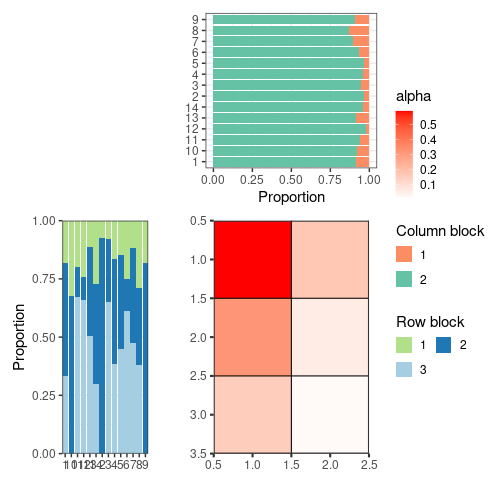
\includegraphics{presentation_dore_files/figure-latex/pirho_meso_plot-9.pdf}
\caption{Collection 9 - pirho}
\end{figure}

\begin{tabular}{l}
\hline
Networks\\
\hline
eberling1999\\
\hline
ramirez1992\\
\hline
Struck1994\\
\hline
Albrecht2010\_49yr+Albrecht2010\_63yr+Albrecht2010\_84yr+Albrecht2010\_109yr+Albrecht2010\_130yr\\
\hline
Devoto2005\_PP+Devoto2005\_AP\\
\hline
Devoto2005\_VT\\
\hline
Gibson2006\_TA2\\
\hline
MonteroCastano2017\_Albufera+MonteroCastano2017\_Llimpa+MonteroCastano2017\_Tirant\\
\hline
Yoshihara2008\\
\hline
PopicThesis\\
\hline
Orford\_B1+Orford\_B2+Orford\_B3+Orford\_B4+Orford\_B5+Orford\_B10\\
\hline
Souza\_vereda\\
\hline
Adedoja2018b\_baseZone+Adedoja2018b\_MidZone+Adedoja2018b\_HighZone+Adedoja2018b\_PeakZone\\
\hline
Hackett2019\_NZ\_salt\_marsh+Hackett2019\_NZ\_sand\_dune+Hackett2019\_NZ\_scrub\_coprosma\\
\hline
\end{tabular}

Pour la collection 10

\begin{figure}
\centering
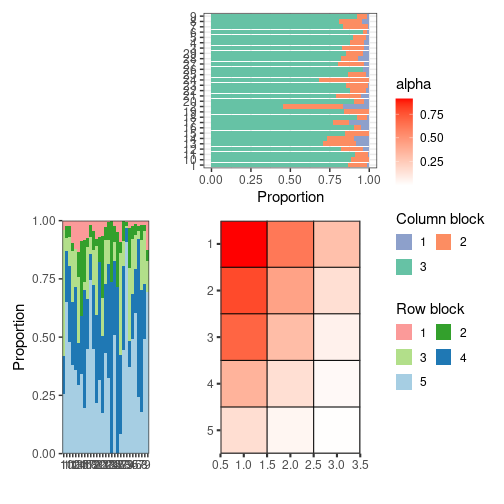
\includegraphics{presentation_dore_files/figure-latex/pirho_meso_plot-10.pdf}
\caption{Collection 10 - pirho}
\end{figure}

\begin{tabular}{l}
\hline
Networks\\
\hline
herrera1988\\
\hline
Burkle2013\\
\hline
bartomeus2008\\
\hline
Olito-Fox2014\\
\hline
Benadi2013\_4(1700m)+Benadi2013\_5(1800m)\\
\hline
Baldock2011\_TB+Baldock2011\_JN\\
\hline
Chamberlain\_HLU+Chamberlain\_HLG+Chamberlain\_OKU+Chamberlain\_OKG+Chamberlain\_WLU+Chamberlain\_WLG+Chamberlain\_SOU+Chamberlain\_SOG\\
\hline
Chamberlain\_Site1+Chamberlain\_Site2+Chamberlain\_Site3+Chamberlain\_Site4+Chamberlain\_Site5+Chamberlain\_Site6\\
\hline
Devoto2005\_LQ\\
\hline
Devoto2005\_LT+Devoto2005\_LH\\
\hline
Devoto2005\_LL+Devoto2005\_CT\\
\hline
Dupont2009\_IsenBjerg+Dupont2009\_Other\\
\hline
Gibson2006\_GA1\\
\hline
LaraRomero2016\_pe?alara\_EP+LaraRomero2016\_pe?alara\_PA+LaraRomero2016\_nevero\_EP+LaraRomero2016\_nevero\_PA\\
\hline
Marrero2013\\
\hline
Trojelsgaard2015\_Tenerife Teno Bajo+Trojelsgaard2015\_Tenerife Fasnia\\
\hline
Vanbergen2013\_balfarm+Vanbergen2013\_bridgend+Vanbergen2013\_dalhaikie+Vanbergen2013\_netherton+Vanbergen2013\_backhill+Vanbergen2013\_corntulloch+Vanbergen2013\_allancreich\\
\hline
Fragoso\_RA2+Fragoso\_RA3+Fragoso\_RD1+Fragoso\_RD3\\
\hline
Pornon2017\\
\hline
Orford\_B6+Orford\_B7+Orford\_B8+Orford\_B9\\
\hline
Blumel2016\\
\hline
Kantsa2018\\
\hline
Grass2013\_1+Grass2013\_2+Grass2013\_3+Grass2013\_4+Grass2013\_5+Grass2013\_6+Grass2013\_7+Grass2013\_8+Grass2013\_9+Grass2013\_10+Grass2013\_11+Grass2013\_12+Grass2013\_13+Grass2013\_14+Grass2013\_15+Grass2013\_16+Grass2013\_17\\
\hline
CordenizPicanco2018\_NatVeg\\
\hline
Hackett2019\_UK\_sand\_dune+Hackett2019\_UK\_grassland+Hackett2019\_UK\_heathland+Hackett2019\_UK\_woodland+Hackett2019\_UK\_salt\_marsh+Hackett2019\_UK\_scrub\\
\hline
Traveset2013\_Pinta\\
\hline
Traveset2013\_SanCristobal\\
\hline
Simanonok2014\\
\hline
Baldock2019\_Edinburgh\\
\hline
\end{tabular}

Pour la collection 11

\begin{figure}
\centering
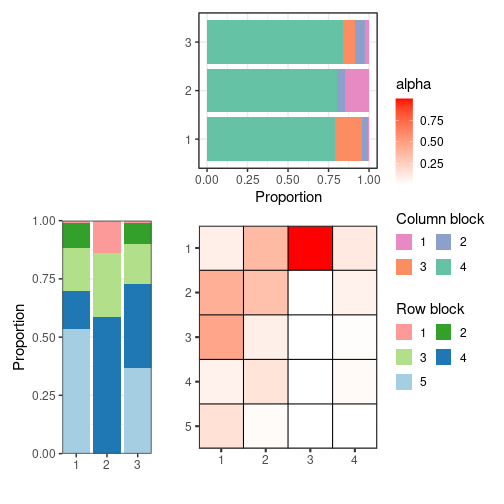
\includegraphics{presentation_dore_files/figure-latex/pirho_meso_plot-11.pdf}
\caption{Collection 11 - pirho}
\end{figure}

\begin{tabular}{l}
\hline
Networks\\
\hline
kato1990\\
\hline
ramirez1989\\
\hline
Kato1993\\
\hline
\end{tabular}

Pour la collection 12

\begin{figure}
\centering
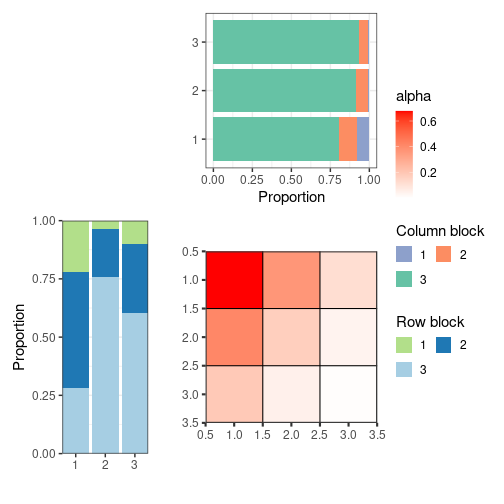
\includegraphics{presentation_dore_files/figure-latex/pirho_meso_plot-12.pdf}
\caption{Collection 12 - pirho}
\end{figure}

\begin{tabular}{l}
\hline
Networks\\
\hline
Chamberlain\_cr1+Chamberlain\_cr2+Chamberlain\_fs1+Chamberlain\_fs2+Chamberlain\_go1+Chamberlain\_go2+Chamberlain\_mm1+Chamberlain\_mm2+Chamberlain\_mz1+Chamberlain\_mz2+Chamberlain\_sm1+Chamberlain\_sm2\\
\hline
Dattilo2016\\
\hline
KatoMiura1996\\
\hline
\end{tabular}

Pour la collection 13

\begin{figure}
\centering
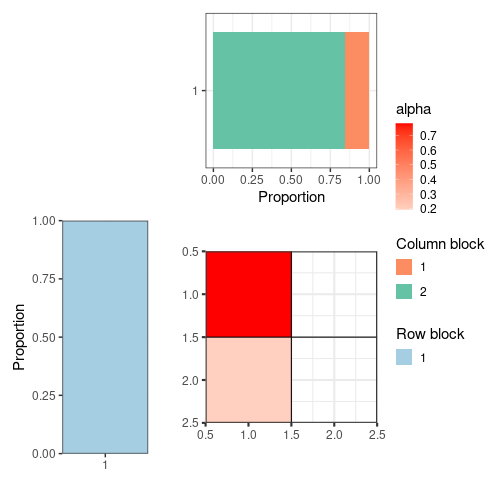
\includegraphics{presentation_dore_files/figure-latex/pirho_meso_plot-13.pdf}
\caption{Collection 13 - pirho}
\end{figure}

\begin{tabular}{l}
\hline
Networks\\
\hline
olensen2002aig\\
\hline
\end{tabular}

Pour la collection 14

\begin{figure}
\centering
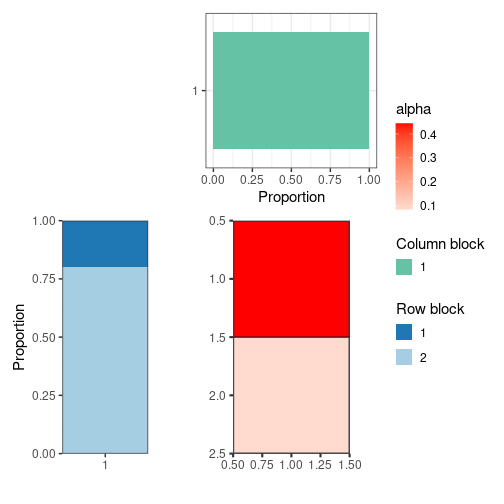
\includegraphics{presentation_dore_files/figure-latex/pirho_meso_plot-14.pdf}
\caption{Collection 14 - pirho}
\end{figure}

\begin{tabular}{l}
\hline
Networks\\
\hline
Trojelsgaard2015\_El Hierro\\
\hline
\end{tabular}

Pour la collection 15

\begin{figure}
\centering
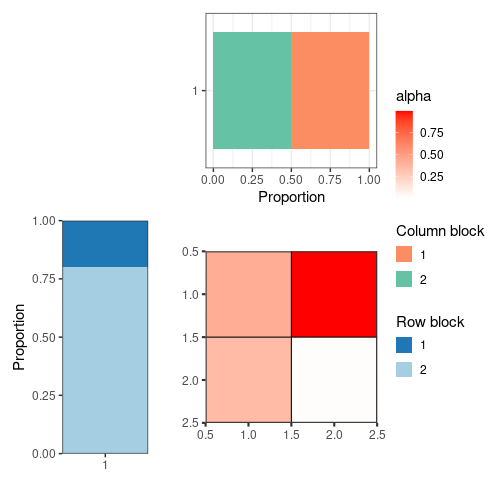
\includegraphics{presentation_dore_files/figure-latex/pirho_meso_plot-15.pdf}
\caption{Collection 15 - pirho}
\end{figure}

\begin{tabular}{l}
\hline
Networks\\
\hline
Gibson2006\_GA2\\
\hline
\end{tabular}

Et voici donc les valeurs numériques pour les \(\alpha\) (paramètres de
connectivité).

Pour la collection 1 :
\[\begin{bmatrix} 0.52 &0.6 &0.34 &0.1 &0.15 &0 &0.36 \\0.12 &0.93 &0.01 &0.01 &0 &0.61 &0.16 \\0.05 &0.31 &0.02 &0.08 &0.37 &0.27 &0.12 \\0.04 &0.05 &0.01 &0.38 &0.03 &0.01 &0.17 \\0 &0.03 &0.16 &0.11 &0.04 &0.01 &0.01 \\0.01 &0.22 &0.02 &0.01 &0.05 &0 &0.01 \\ \end{bmatrix}\]
Pour la collection 2 :
\[\begin{bmatrix} 0.66 &0.23 \\0.2 &0.05 \\ \end{bmatrix}\] Pour la
collection 3 :
\[\begin{bmatrix} 0.64 &0.32 &0.11 &0.53 &0.19 &0.05 \\0.47 &0.21 &0.02 &0.19 &0.07 &0.03 \\0.16 &0.05 &0.01 &0.07 &0.01 &0 \\ \end{bmatrix}\]
Pour la collection 4 :
\[\begin{bmatrix} 0.45 &0.07 \\0.22 &0.62 \\0.23 &0.04 \\ \end{bmatrix}\]
Pour la collection 5 :
\[\begin{bmatrix} 0.78 &0.43 &0.16 &0.56 \\0.29 &0.04 &0.22 &0.08 \\0.02 &0.12 &0.03 &0 \\ \end{bmatrix}\]
Pour la collection 6 :
\[\begin{bmatrix} 0.82 &0.63 &0.2 &0.74 \\0.34 &0.07 &0.41 &0.13 \\0.02 &0.16 &0.03 &0 \\ \end{bmatrix}\]
Pour la collection 7 :
\[\begin{bmatrix} 0.9 &0.46 &0.72 \\0.17 &0.37 &0.03 \\ \end{bmatrix}\]
Pour la collection 8 :
\[\begin{bmatrix} 0.66 &0.97 &0.72 &1 &0.13 &0.71 &0 \\0.99 &0.93 &0.84 &0.64 &0.5 &0.11 &0.17 \\0.71 &0.7 &0.28 &0.32 &0.13 &0.07 &0.05 \\0.96 &0.46 &0.75 &0.14 &0.39 &0.01 &0.07 \\0.62 &0.36 &0.09 &0.11 &0.04 &0.02 &0.01 \\0.62 &0.12 &0.43 &0.02 &0.17 &0 &0.02 \\0.33 &0.03 &0.14 &0 &0.03 &0 &0 \\ \end{bmatrix}\]
Pour la collection 9 :
\[\begin{bmatrix} 0.59 &0.17 &0.32 \\0.06 &0.15 &0.02 \\ \end{bmatrix}\]
Pour la collection 10 :
\[\begin{bmatrix} 0.91 &0.62 &0.3 &0.79 &0.44 \\0.15 &0.7 &0.32 &0.07 &0.36 \\0.15 &0.03 &0.16 &0.05 &0.01 \\ \end{bmatrix}\]
Pour la collection 11 :
\[\begin{bmatrix} 0.09 &0.36 &1 &0.12 &0.41 \\0.33 &0 &0.07 &0.46 &0.09 \\0 &0.01 &0.07 &0.14 &0 \\0.03 &0.16 &0.02 &0 &0 \\ \end{bmatrix}\]
Pour la collection 12 :
\[\begin{bmatrix} 0.68 &0.37 &0.12 \\0.41 &0.17 &0.04 \\0.19 &0.05 &0.01 \\ \end{bmatrix}\]
Pour la collection 13 : \[\begin{bmatrix} 0.78 \\0.19 \\ \end{bmatrix}\]
Pour la collection 14 : \[\begin{bmatrix} 0.44 &0.08 \\ \end{bmatrix}\]
Pour la collection 15 :
\[\begin{bmatrix} 0.42 &1 \\0.35 &0.01 \\ \end{bmatrix}\]

\hypertarget{ruxe9partition-dans-les-clusters-selon-la-taxonomie-3}{%
\subsubsection{Répartition dans les clusters selon la
taxonomie}\label{ruxe9partition-dans-les-clusters-selon-la-taxonomie-3}}

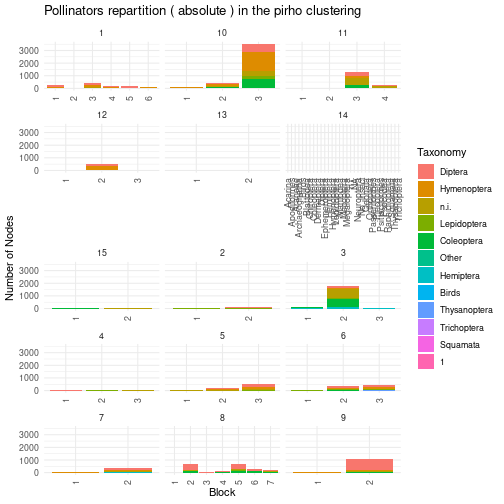
\includegraphics{presentation_dore_files/figure-latex/pirho_plot_taxonomy_pollinators-1.pdf}
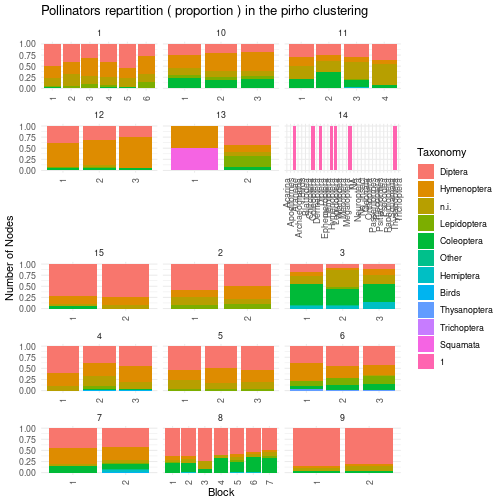
\includegraphics{presentation_dore_files/figure-latex/pirho_plot_taxonomy_pollinators-2.pdf}

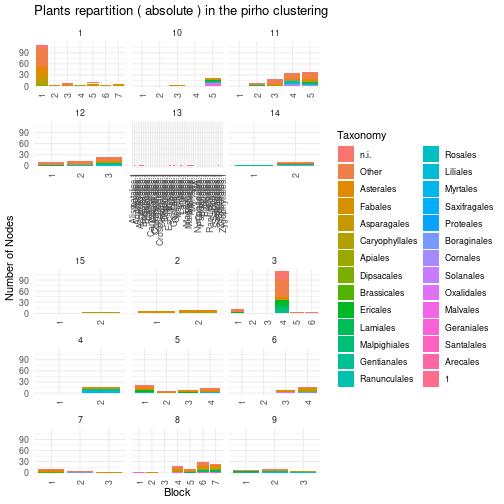
\includegraphics{presentation_dore_files/figure-latex/pirho_plot_taxonomy_plants-1.pdf}
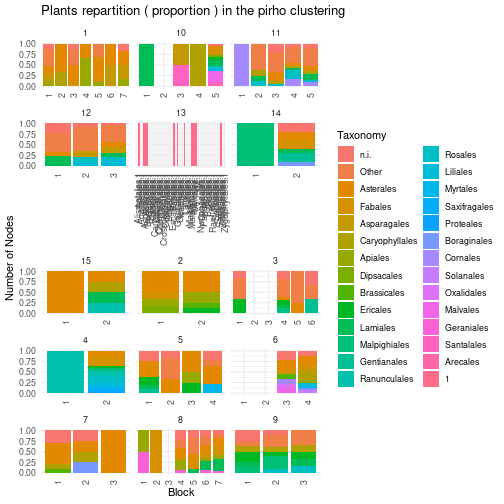
\includegraphics{presentation_dore_files/figure-latex/pirho_plot_taxonomy_plants-2.pdf}

\end{document}
